%Lens optics
At your childhood you may have the experience by using a magnifiying glass to set small pieces of paper or leaves on fire with sunlight. The lens of the manifying glass focuses all incoming light tays at a single point. espeically for the rays parallel with the lens' axis the single point of the lens is called focal point and the distance between the focal point and the center of the lens is called focal length $f$.
The focal length of a lens depends on the radii of curvature of its surface and on the index of the refraction of the material the lens is made from. In oder to undertand more specifics about lenses a singlet lens with geometric parameters is presented in Fig.\ref{fig:lens_define}.

\begin{figure}[httbp]
\centering
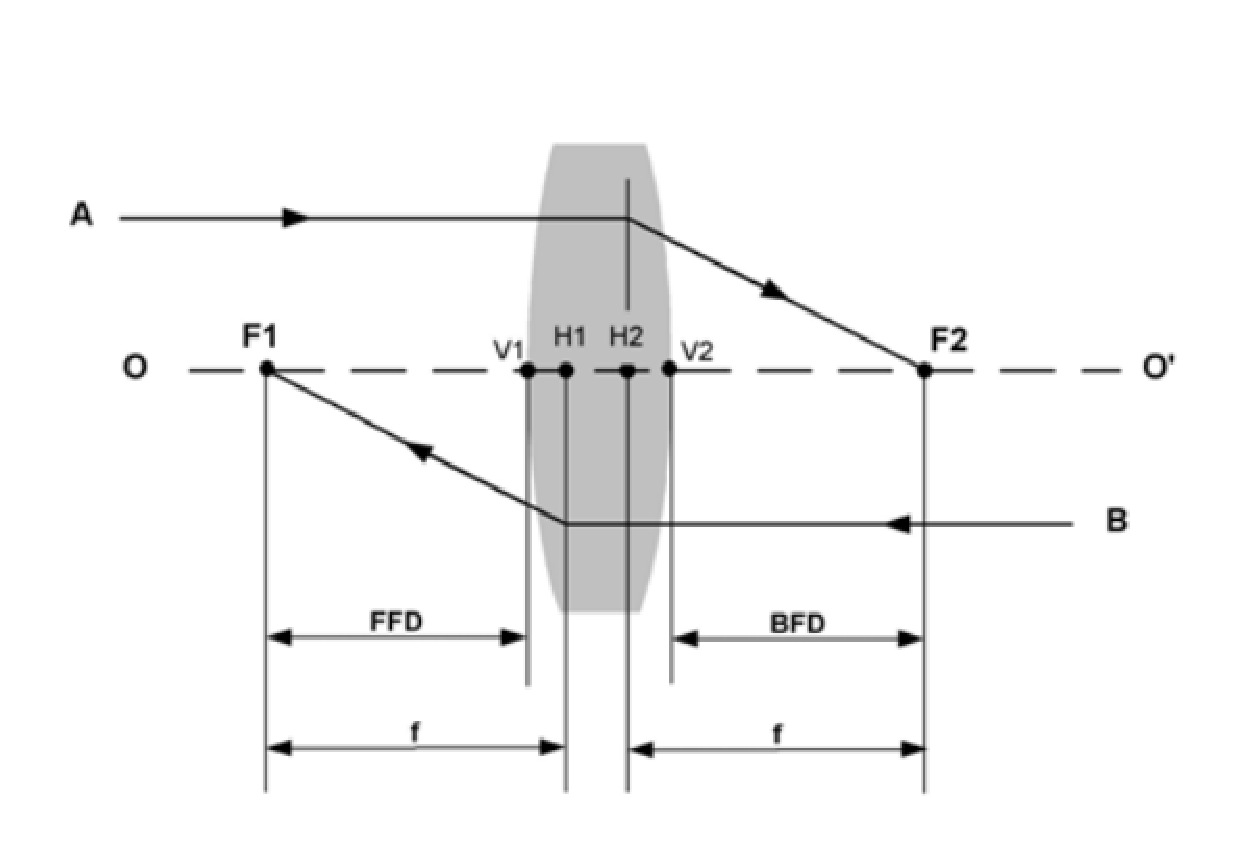
\includegraphics[width=0.33\textwidth]{bilder/lens_define}
\caption{The quantities define of singlet lenses}
\label{fig:lens_define}
\end{figure}

The optical axis (O-O')of the lens is a line passing through the centers of curvature of the two spherical lens surfaces. 
Rays A and B,parallel with the optic axis (O-O'), are  casted from different two sides through the lens and respectively cross the axis at their front and back focal points $F1$ and $F2$. The front and back principal points $H1$ and $H2$ are the intersections of the optical axis with the front and back principal surfaces. Points $V1$ and $V2$ are called the front and back vertices respectively. So important Quantities are defined in the Tab.\ref{tab:lens_quantities}.


\begin{table}
\begin{tabular}{|c|c|c|}
\hline
\textbf{Symbol}&\textbf{Description}&\textbf{Formular}\\
\hline
$f$ & \parbox[c]{6cm}{
						\begin{center}
						effective focal length
						\end{center}
				}& $\frac{1}{f}=(n-1)\left[\frac{1}{R_{1}}-\frac{1}{R_{2}} \right]+\frac{t_{c}(n-1)^2}{nR_{1}R_{2}}$ \\
\hline
$BFD$ &\parbox[c]{6cm}{
						\begin{center}
						back focal distance 
						\end{center}
			}& $BFD=f\left[ 1-\frac{t_{c}(n-1)}{nR_{1}}\right]$ \\
\hline
$FFD$ &\parbox[c]{6cm}{
						\begin{center}
						 front focal distance
						 \end{center} 
			}& $FFD=f\left[ 1+\frac{t_{c}(n-1)}{nR_{1}}\right]$ \\
\hline
$H2V2$ & \parbox[c]{6cm}{
						\begin{center}
						back vertex to back principal point distance
						\end{center}						
			} & $H_{2}V_{2}=f-BFD=-f\frac{t_{c}(n-1)}{nR_{1}}$ \\
\hline
$V1H1$ & \parbox[c]{6cm}{
						\begin{center}			
				    front vertex to front principal point distance
				    \end{center}
				 } & $V_{1}H_{1}=f-FFD=-f\frac{t_{c}(n-1)}{nR_{2}}$ \\
\hline
\end{tabular}
\caption{Important Quantities for Singlet Lenses Immersed in Air}
\label{tab:lens_quantities}
\end{table}


The distance $t_{c}$ is the center thinckness of the lens $V1V2$. 






The classical singlet lenses are plano convex, plano concave, equiconvex and equiconcave lenses, which are listed in following Tab.\ref{tab:lenses_focal_length} with their focal lengths.

\begin{table}
\begin{tabular}{|c|c|c|}
\hline
\textbf{Type}&\textbf{Description}&\textbf{Formular}\\
\hline
Plano Convex & \parbox[c]{2.1cm}{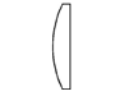
\includegraphics[width=2cm]{bilder/plano_convex}}& $f=\frac{R}{(n-1)}$ \\
\hline
Plano Concave &\parbox[c]{2.1cm}{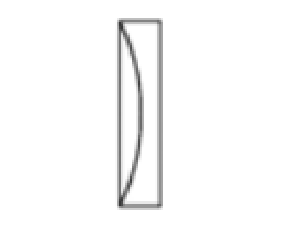
\includegraphics[width=2cm]{bilder/plano_concave}} & $f=-\frac{R}{(n-1)}$ \\
\hline
Equiconvex & \parbox[c]{2.1cm}{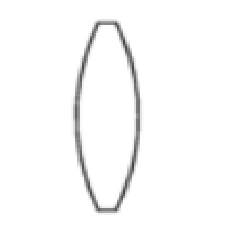
\includegraphics[width=2cm]{bilder/equi_convex}} & $f=\left[\frac{2(n-1)}{R} - \frac{t_{c}(n-1)^2}{nR^2}\right]^{-1}$ \\
\hline
Equiconcave & \parbox[c]{2.1cm}{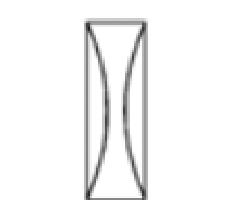
\includegraphics[width=2cm]{bilder/equi_concave}} & $f=\left[\frac{2(n-1)}{R} + \frac{t_{c}(n-1)^2}{nR^2}\right]^{-1}$ \\
\hline
\end{tabular}
\caption{Focal length Formulas of Simple Singlet Lenses in Air.  
				 The Radii are considered positive in the formulas below.}
\label{tab:lenses_focal_length}
\end{table}


High quality singlet lensese are of particular interest in laser focusing and beam handling applications because of their low cost, high damage threshold, and availability of a large variety of standard parts. ..................
	